\newpage
\section{Evaluation}
\label{sec:evaluation}
\subsection{Determination of the Threshold Current}
As stated in \ref{sec:threshold} the current is slowly raised.
\autoref{fig:laser_before} shows the photo of the light spot before the current exceeds the threshold current.
\autoref{fig:laser_after} shows the record of the laser light at the threshold current $I_\text{th} = 37,0 \,$mA.
\begin{figure}[ht]
    \centering
    \begin{subfigure}{0.49\textwidth}
        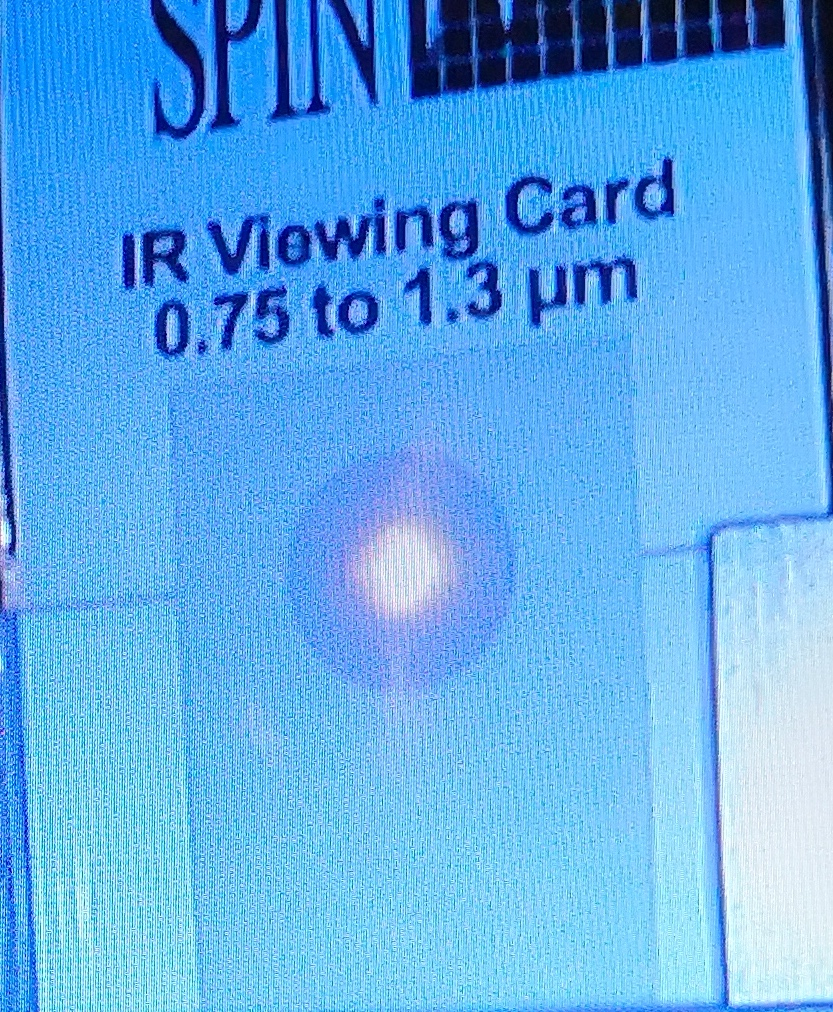
\includegraphics[width=\textwidth]{bilder/laser_before.jpg}
        \caption{The light spot on the card before lasing happens at a current below $I_\text{th}$. \cite{anleitungHeNe}}
        \label{fig:laser_before}
    \end{subfigure}
    \hfill
    \begin{subfigure}{0.49\textwidth}
        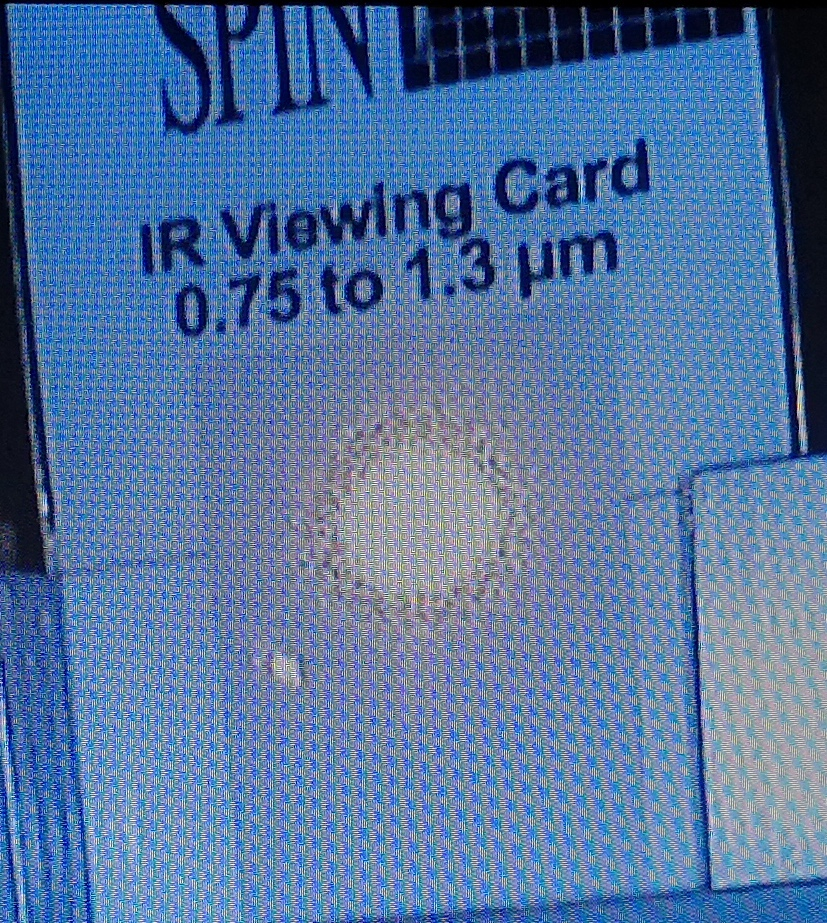
\includegraphics[width=\textwidth]{bilder/laser_after.jpg}
        \caption{The light spot on the card at the threshold current $I_\text{th}$. The laser granulation is seen on the card. \cite{anleitungHeNe}}
        \label{fig:laser_after}
    \end{subfigure}
    \caption{The light spot caused by the diode laser before and after lasing.}
\end{figure}

\FloatBarrier

\subsection{Rubidium fluorescence}
The picture in \autoref{fig:fluorescence} was taken of the rubidium cell as the fluorescence could be seen at all times albeit it was a bit dim.
\begin{figure}[ht]
    \center
    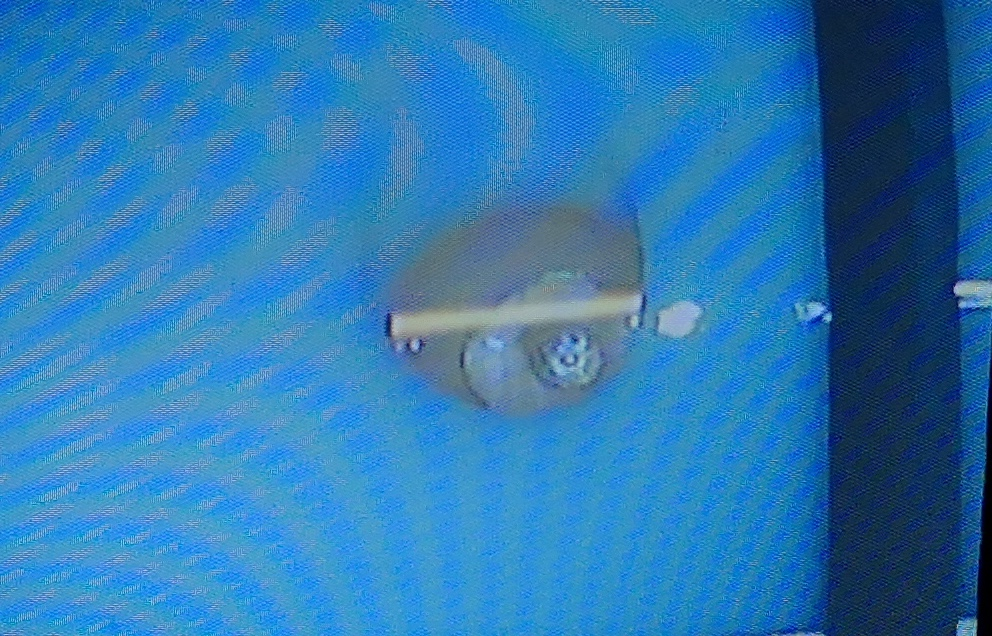
\includegraphics[width=0.65\textwidth]{bilder/fluorescence.jpg}
    \caption{The rubidium fluorescence which is seen when the diode laser reaches the necessary energy to excite the rubidium gas. \cite{anleitungHeNe}}
    \label{fig:fluorescence}
\end{figure}

\FloatBarrier

\subsection{Absorption spectrum of Rubidium}
In \autoref{fig:spectrum} the absorption spectrum of rubidium is shown after the fine adjustment mentioned in \ref{sec:threshold} which involves varying the current, the piezo voltage and the side knob in turn.
From left to right the absorption peaks belong to the transitions 87b, 85b, 85a and 87a.
The blue graph in \autoref{fig:spectrum} signifies a sweep of the piezo.
\begin{figure}[ht]
    \center
    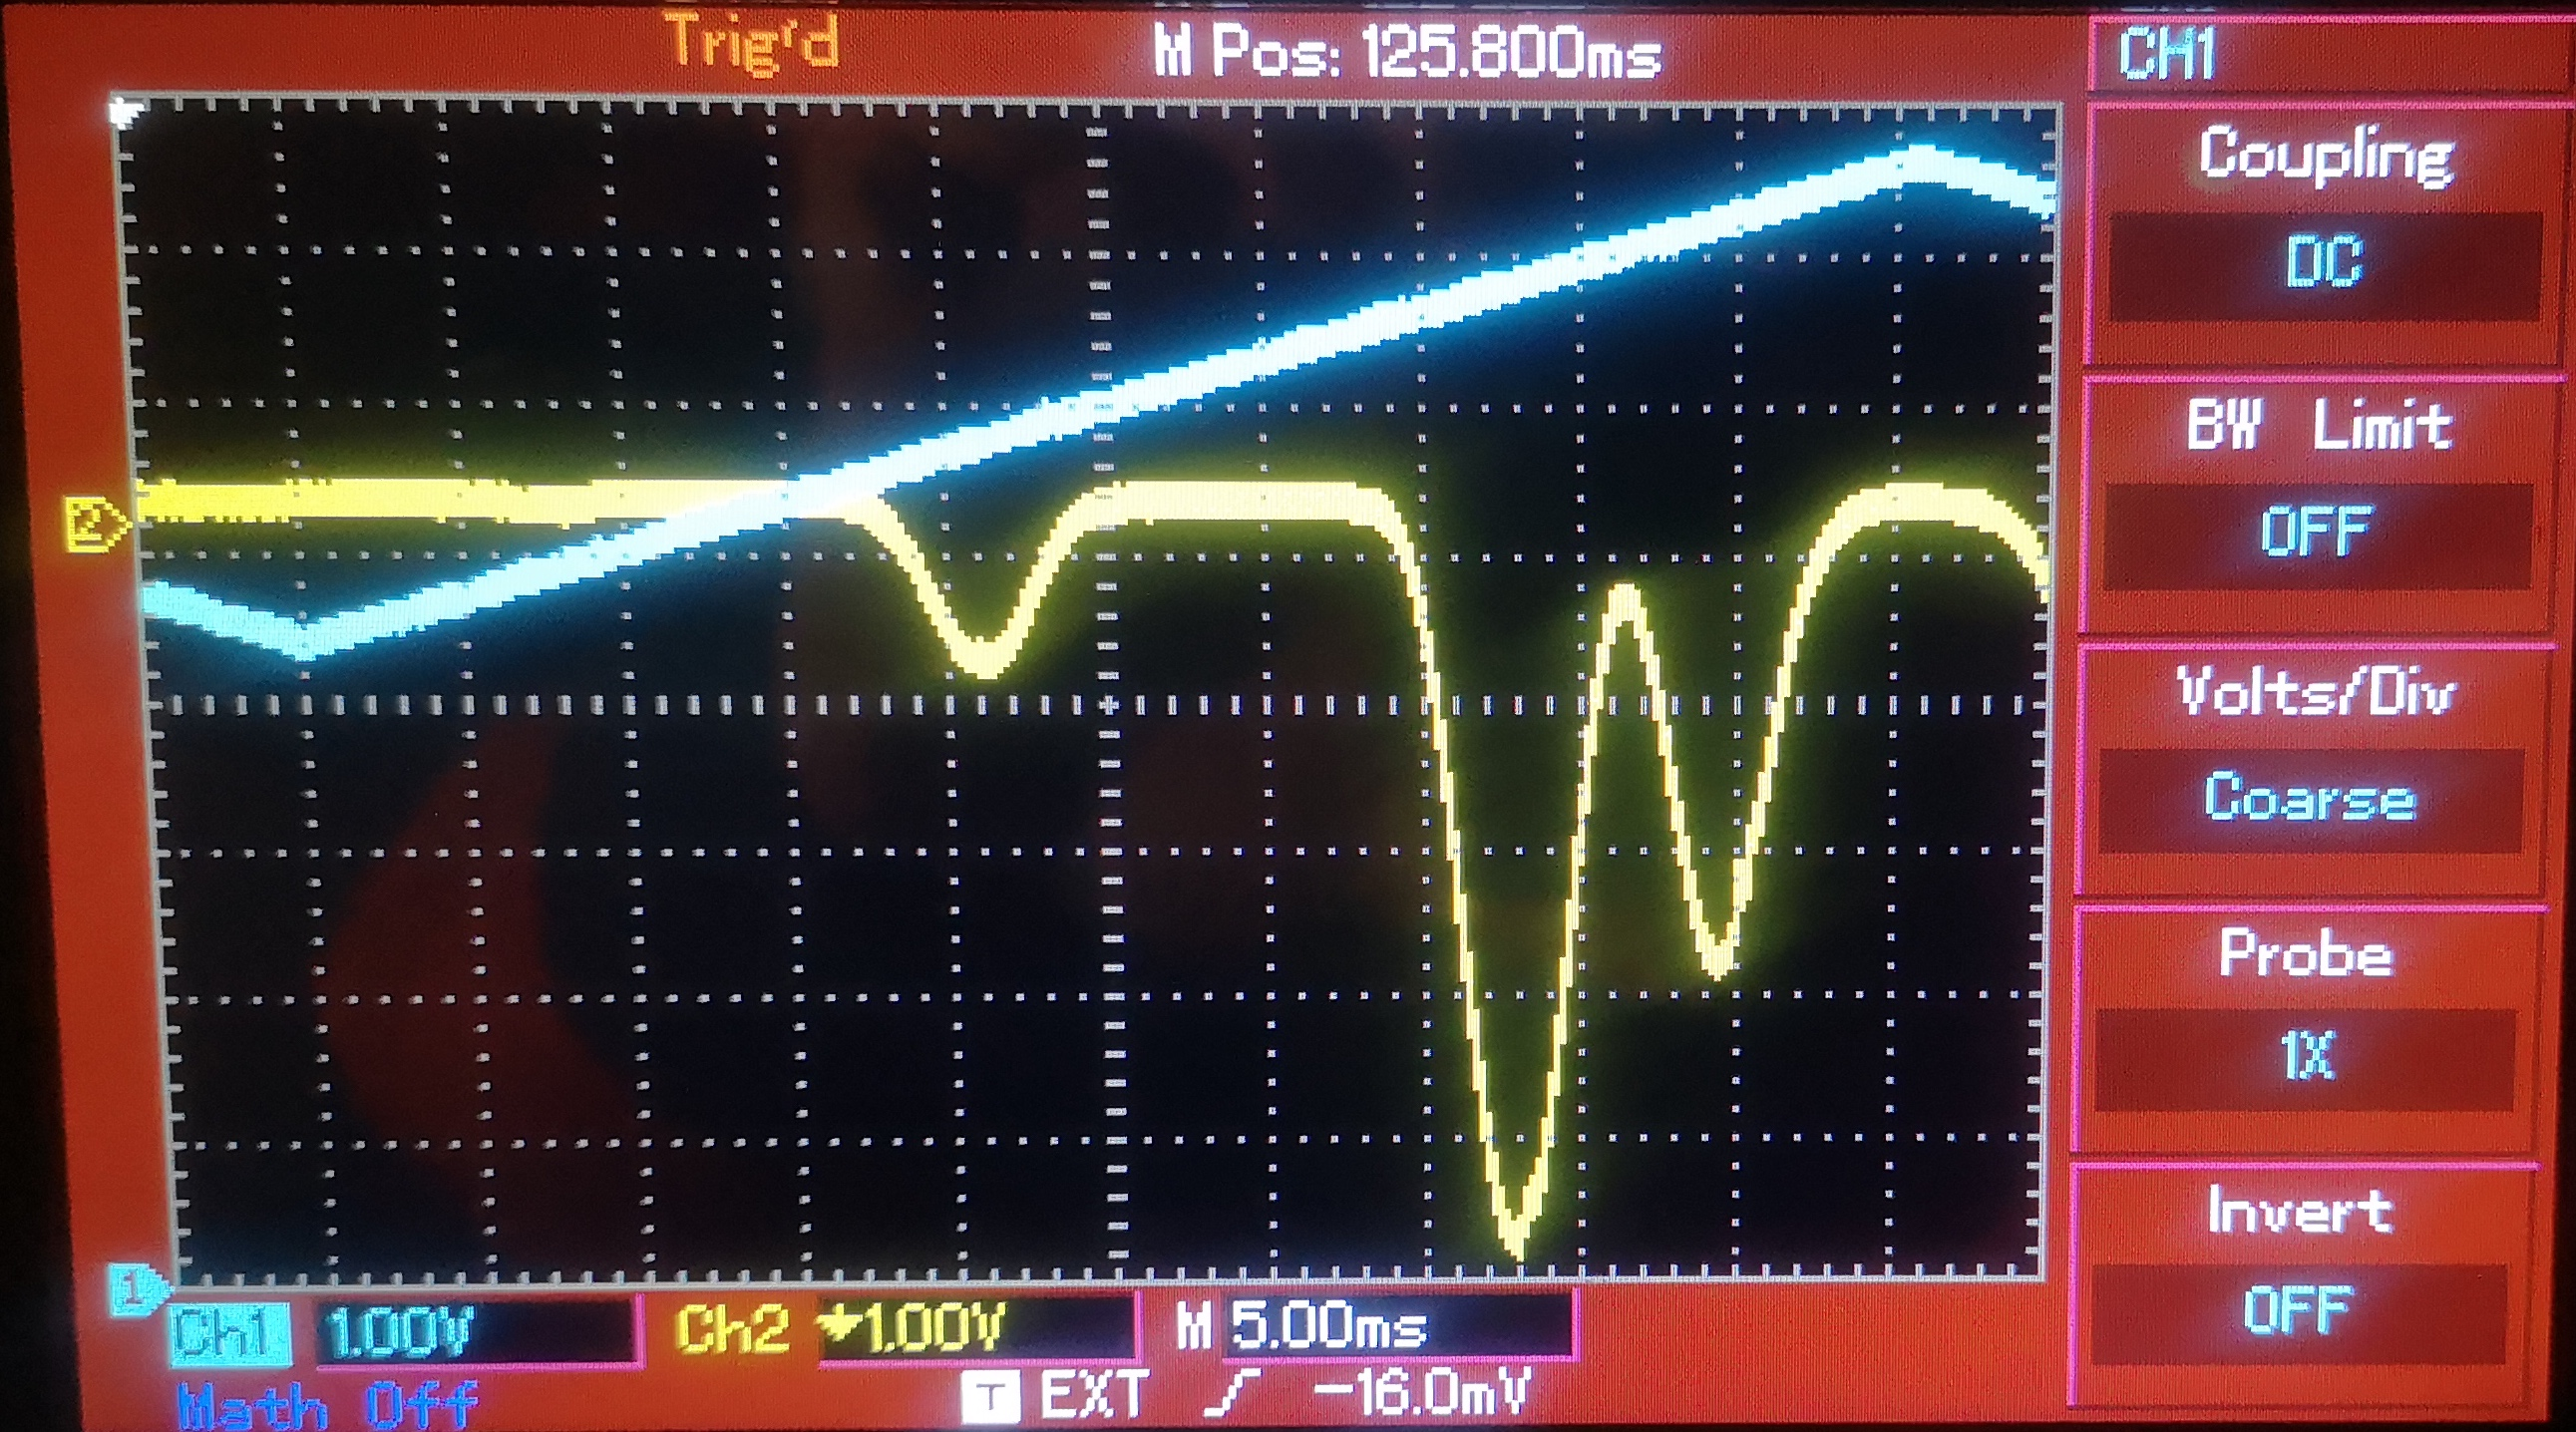
\includegraphics[width=0.75\textwidth]{bilder/spectrum.jpg}
    \caption{The absorption spectrum of rubidium containing the peaks belonging to 85a, 85b, 87a and 87b after the adjustment of the laser parameters. \cite{anleitungHeNe}}
    \label{fig:spectrum}
\end{figure}

\FloatBarrier